\section{Semana 4 - Design Point}
A semana quatro foi focada plenamente na procura dum design point válido.\par
Considere-se o Peso da aeronave projetada, W,a área de superfície da Asa, S, a Potência disponível, P, e a Área . A procura foi caracterizada por utilizar o programa disponibilizado e alterar os valores de forma a alterar os rácios: W/S, W/P e W/A. Desta forma, procurou-se encontrar um equilíbrio entre as dimensões da aeronave, a missão e os motores. Além de tal, teve-se em conta o grau de realismo dos valores ao se comparar com aqueles de aeronaves já concebidas, dado que o programa não consegue distinguir para casos irreais/contraditórios e que certos valores de diretamente relacionados com a performance são hardcoded no json, como o "power" dos motores elétricos.\par
\subsection{Descrição e Implementação}
É importante, primeiramente, dar uma breve descrição da aeronave, de forma a ser possível entender certas restrições tomadas, bem como esclarecer qual os cuidados tidos a implementá-la no programa.\par
\FloatBarrier
\begin{figure}[h]
    \centering
    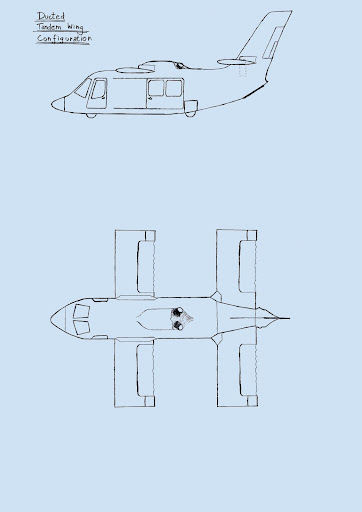
\includegraphics[width=0.4\textwidth]{Imagens/segundodesign2.jpg}
    \caption{Desgin escolhido}
    \label{designescolhido}
\end{figure}
\FloatBarrier
Baseado no AHP, foi escolhido o design apresentado em \ref{designescolhido}, em cima.\par
Este design apresenta tandem wing, com as asas desniveladas, de forma a diminuir a interferência. Nesta fase do design, o fator de interferência default no programa não foi mudado dada a ainda não realizada procura de relações empíricas. Além de tal, de forma a implementar a tandem wing, foi considerado que o o componente "Horizontal Tail" presente no ficheiro json de input para o programa poderia ser mudada de forma a ter a envergadura e corda necessário. Tal será mudado em futuras semanas, após ser descoberto como o programa calcula a área S e o lift nos cálculos de desempenho necessários para a estimação de combustível em cada troço, por análise direta do source code. A cauda de horizontal não é tratada como uma asa no código, não contribuindo para os cálculos do lift e do desempenho como se fosse uma asa principal, desprezando-se assim contribuíções que se tornam relevantes quando a as dimensões são comparáveis (neste caso iguais) às da asa principal.\par
Deve-se adicionar que as superfícies de controlo normalmente encontradas numa estabilizador horizontal encontram-se na asa posterior (de trás), utilizando-se, então, a configuração usual.\par
Em relação à propulsão, baseado no Lillium Jet, foi considerada uma distribuída, sobre a asa, no bordo de fuga. Esta é baseada em ter um motor com uma hélice cada ambos dentro de ductos convergentes. Não foi considerado utilizar um menor número de motores com maior potência, possivelmente colocados dentro da fuselagem, cada um alimentando várias hélices, dada a complexidade adicional na transmissão, que adiciona tanto peso como maior possibilidade de falha, É projetado, inicialmente, que existam cerca de 20 a 30 motores elétricos, dado que o Lillium Jet possui 36\cite{noauthor_2021-sz}. Diminuição do ruído, esteiras convergentes e os menores números de Mach locais devido aos ductos, o que permite maiores velocidades de rotação, (em comparação com sem ductos) são considerados como vantagens que deverão sobrepor-se ao atrito e ao peso impostos pela estrutura adicional necessária. Para ter estes em conta no programa, foi, nesta fase do projeto, apenas caracterizado os parâmetros já presentes no programa, nomeadamente, a quantidade, o raio, o número de pás, a velocidade, a massa, a eficiência e a potência. Tal foi devido a ser considerado que implementar um design mais realista só faria sentido numa fase mais avançada, nomeadamente, após se conseguir ter a versão simplificada a funcionar com valores plausiveis, dado que a tanto a procura de dados empíricos bem como a sua implementação no programa disponibilizado seria demorada e morosa e, por isso, demasiado custosa, dada a prioridades de ter um primeiro design funcional. É possível verificar a implementação escolhida em \ref{propulsoasemana4json}
\FloatBarrier
\begin{figure}[h]
    \centering
    \begin{subfigure}[h]{0.33\textwidth}
        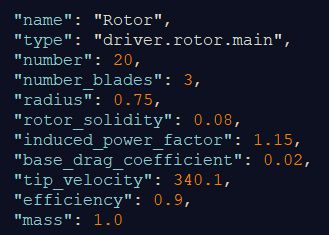
\includegraphics[width=\textwidth]{Imagens/rotor semana 4.PNG}
        \caption{Rotor - semana 4}
        \label{}
    \end{subfigure}
    \hfill
    \begin{subfigure}[h]{0.33\textwidth}
        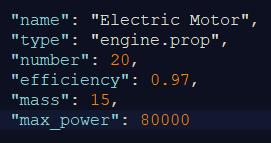
\includegraphics[width=\textwidth]{Imagens/motor semana 4.PNG}
        \caption{Motor elétrico - semana 4}
        \label{}
    \end{subfigure}
    \caption{Implementação da propulsão no ficheiro json - Semana 4}
    \label{propulsoasemana4json}
\end{figure}
\FloatBarrier
Esta escolha de arquitetura de propulsão impôs as seguintes restrições/decisões:
\begin{itemize}
    \item Os rotores deverão ter um diâmetro tal que a soma destes seja menor que a envergadura da asa (ou seja, que haja espaço para os acomodar)
    \item que a corda seja menor que o conjunto rotor + motor. Isto só pode ser tido em conta após ser escolhido o motor
    \item que a corda seja maior que a o diâmetro do rotor, de forma a que as proporções sejam plausíveis e não coloque problemas nem estruturais nem aerodinâmicos
    \item potência dos motores somados menor ou igual à gerada pelos gerados com o turboshaft
\end{itemize}
Para a estimar a massa e potência dos motores elétricos, foi tomada como referência o REB 90 ELECTRIC MOTOR da MGM COMPRO, dado o facto de ser utilizado em aeronáutica. A empresa afirma que é:"Highly variable and customizable, yet very powerful 80 KW electric motor. Suitable for a wide range of aviation projects, such as multirotor applications (UAVs), drones, gliders, as well as various types of marine projects. Tuned especially for complex projects with high demand for compact dimensions and very light weight.".\cite{noauthor_2021-ym}Este tinha 15kg e 80kW de potência\cite{noauthor_2021-ym}. Foi escolhido por ter sido considerado o melhor no mercado atual com as dimensões, tanto de volume como massa, e potência necessárias.\par
Além do descrito explicitamente aqui, este design em tudo se assemelha ao apresentado na semana 1, presente na figura \ref{DesingSketchini1}
\subsection{Design Point}
O Design Point da semana 4, uma primeira aproximação/estimação, foi conseguido ao preencher o json com os valores estimados e procurados iniciais e depois ajustar os valores de forma a conseguir um design considerado possível. Esta avaliação é conseguida com os rácios, já mencionados, W/S, W/P e W/A, e zonas nos gráficos (W/P, W/S) e (W/P,W/A) onde o design, segundo o modelo tomado, funcionaria em todos os troços. Será necessário mencionar, desde já, que apenas a massa total foi retirada do programa, e não a do combustível nem a da bateria nesta semana, devido a desconhecimento desta funcionalidade. Devido a tal, a exequibilidade da missão não foi tida em conta nesse campo, dado que, caso um troço não seja possível devido à mass fraction ter que ser maior que um (situação fisicamente impossível), o programa retorna um valor imaginário como massa de combustível ou de bateria; não retorna, no entanto, qualquer tipo de aviso. Tal é abordado numa semana mais adiante.\par
Este é caracterizado por:\par
\FloatBarrier
\begin{table}[h]
\begin{adjustbox}{width=1\textwidth}
\begin{tabular}{|l|l|lll}
\cline{1-2}
Crew (100 kg/person)       & 2 tripulantes - 200 kg                            &                       &                               &                                                                   \\ \cline{1-2} \cline{4-5} 
Passengers (100 kg/person) & 5 passageiros - 500 kg                            & \multicolumn{1}{l|}{} & \multicolumn{1}{l|}{Rotor}    & \multicolumn{1}{l|}{0 kg -2 rotores - 5 pás - 2 metros raio}      \\ \cline{1-2} \cline{4-5} 
Avionics                   & 24 kg                                             & \multicolumn{1}{l|}{} & \multicolumn{1}{l|}{Propeler} & \multicolumn{1}{l|}{50 kg -2 propelers - 4 pás - 2.3 metros raio} \\ \cline{1-2} \cline{4-5} 
Payload Bay                & 200 kg (150 kg medical equipment)                 & \multicolumn{1}{l|}{} & \multicolumn{1}{l|}{Gearbox}  & \multicolumn{1}{l|}{5 kg}                                         \\ \cline{1-2} \cline{4-5} 
Fuselage                   & 1200 kg - 4 metros comprimento - 1 metro diametro &                       &                               &                                                                   \\ \cline{1-2}
Main Wing                  & 840 kg - 7 aspect ratio - 3 metros corda          &                       &                               &                                                                   \\ \cline{1-2}
Horizontal Tail            & 100 kg - 5 aspect ratio - 0.5 metros corda        &                       &                               &                                                                   \\ \cline{1-2}
Vertical Tail              & 50 kg - 5 aspect ratio - 1 metro corda            &                       &                               &                                                                   \\ \cline{1-2}
Turboshaft -               & 0 kg - 210000kW                                   &                       &                               &                                                                   \\ \cline{1-2}
Battery                    & 200 kg - 360000 W/kg                              &                       &                               &                                                                   \\ \cline{1-2}
Generator                  & 924 kg                                            &                       &                               &                                                                   \\ \cline{1-2}
Electric Motor             & 510 kg - 200000W - 3 motores                      &                       &                               &                                                                   \\ \cline{1-2}
Fuel Tank                  & 1200 kg                                           &                       &                               &                                                                   \\ \cline{1-2}
\end{tabular}
\end{adjustbox}
\end{table}
\FloatBarrier
Dever-se-á notar os dados em falta, nomeadamente as massas. Certas massas foram incluídas noutros componetes, como, por exemplo: a massa dos dois turboshafts foi considerada no gerador. Outras, como a dos rotores, ficaram apenas por determinar, posteriormente. Dado a massa inicial de 1200 kg de fuselagem, foi considerado que poder-se-ia discritizar a massa para cada componente numa simulação posterior.\par
O resultado é apresentado de seguida:\par
\FloatBarrier
\begin{figure}[h]
    \centering
    \begin{subfigure}[h]{0.70\textwidth}
        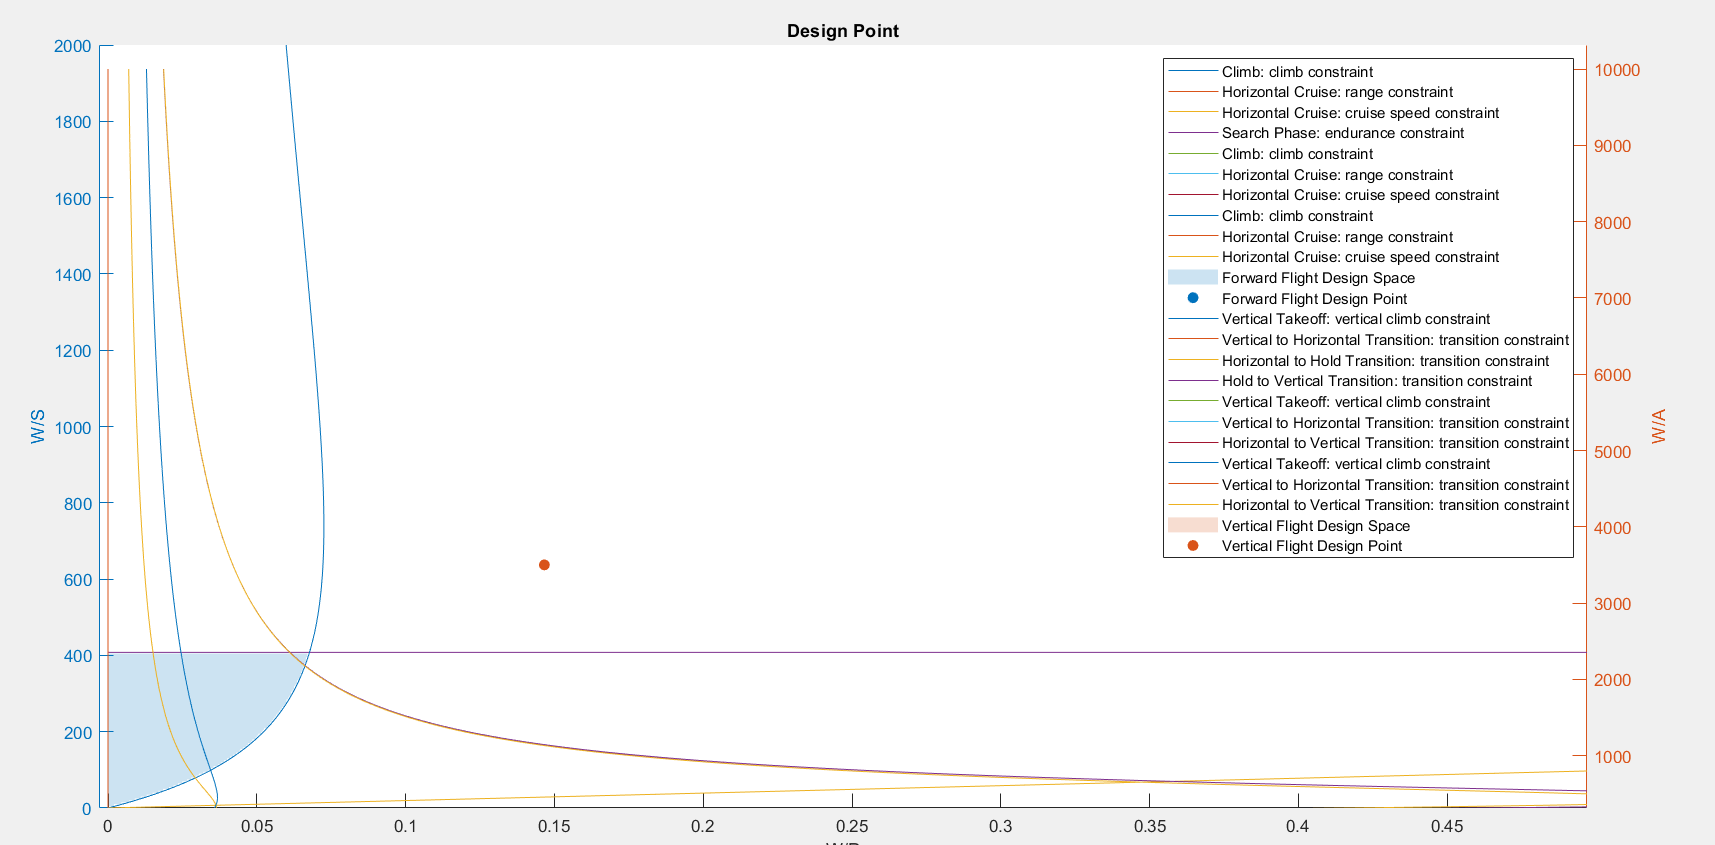
\includegraphics[width=\textwidth]{Imagens/firstplot_designpoint.PNG}
        \caption{Design Point}
        \label{}
    \end{subfigure}
    \hfill
    \begin{subfigure}[h]{0.70\textwidth}
        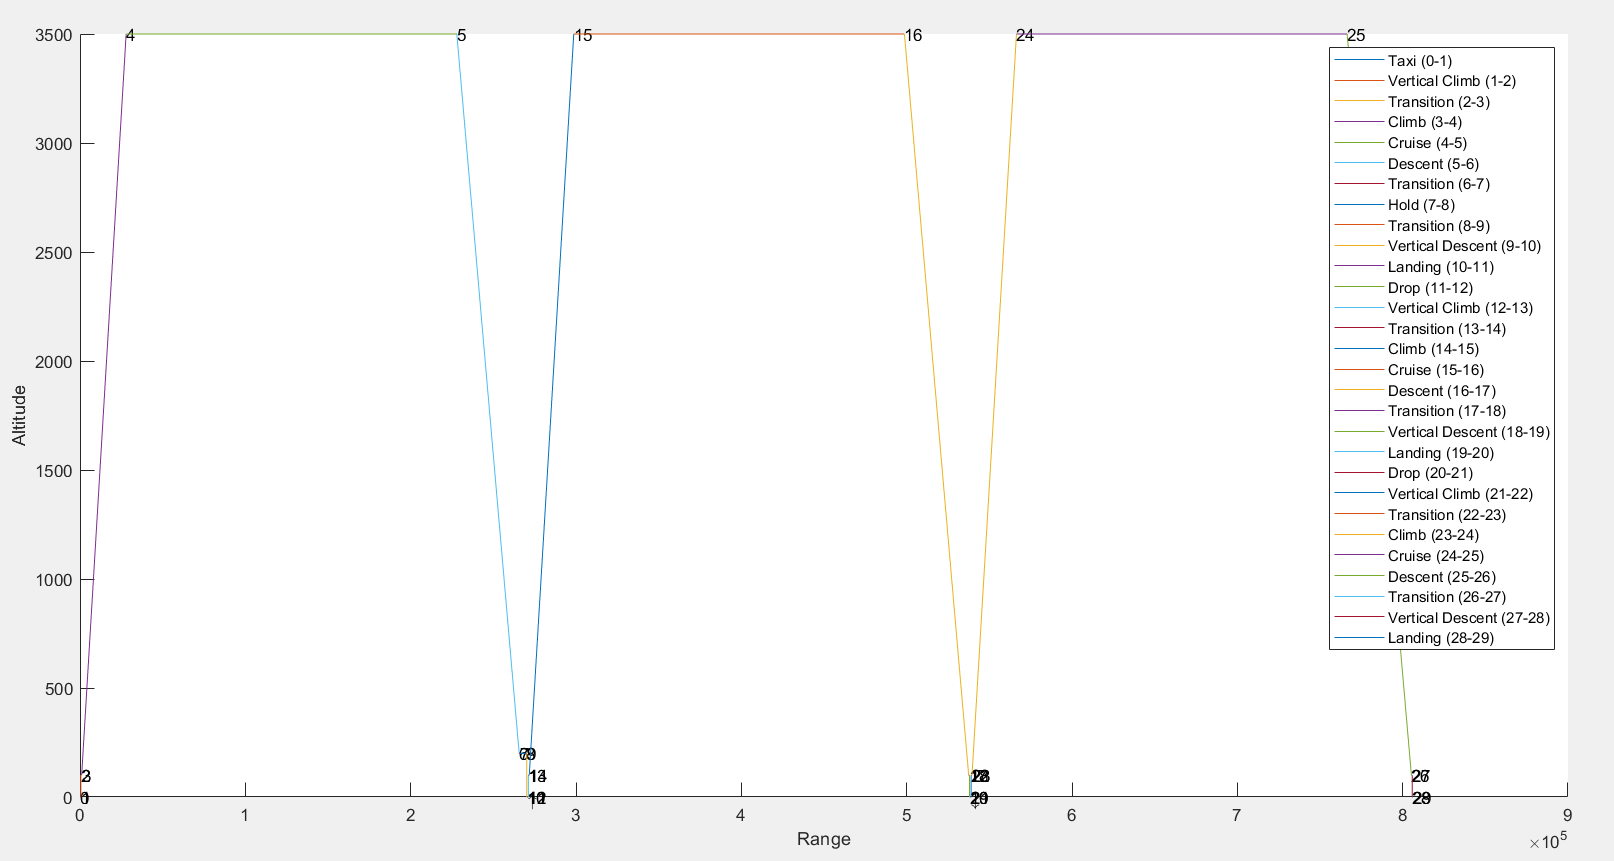
\includegraphics[width=\textwidth]{Imagens/firstplot_mission.PNG}
        \caption{Missão}
        \label{}
    \end{subfigure}
    \caption{Primeiro Plot gerado pelo programa}
    \label{firstplot}
\end{figure}
\FloatBarrier
Imediatamente, foi possível verificar dois aspetos: existem menos linhas no gráfico de design point que o número de troços; e a missão aparenta conter todos os troços corretamente. Esta ultíma afirmação é verdade.\par
Uma inspeção mais atenta, revelou que o menor número de linhas se deve não só a faltarem gráficos mas também a existirem linhas sobrepostas, ou quase sobrepostas, devido a existirem troços com as mesmas características.\par
Uma outra caracteristica importanto que foi logo notada é a de não ter sido formada área laranja, o que significava que existia uma falha na definição ou do veículo ou num troço vertical, não gerando linhas suficientes, dando erro, ou gerando uma na vertical que leva  a área laranja para zero.\par
O json foi alterado de forma a ter agora as seguintes características, mais credíveis:\par
\FloatBarrier 
 \begin{table}[h] 
 \begin{adjustbox}{width=1\textwidth} 
 \begin{tabular}{|c|c|c|c|}
 \hline 

\makecell{name: Crew ; \\ type: mass.point ; \\ mass: 200 ; \\ } & \makecell{name: Passengers ; \\ type: mass.point ; \\ mass: 500 ; \\ } & \makecell{name: Avionics ; \\ type: mass.point ; \\ mass: 5 ; \\ } & \makecell{name: Payload Bay ; \\ type: mass.point ; \\ mass: 10 ; \\ }\\ \hline \\ 
\makecell{name: Fuselage ; \\ type: fuselage ; \\ interf\_factor: 1.0 ; \\ diameter: 1.0 ; \\ length: 4.0 ; \\ mass: 800 ; \\ } & \makecell{name: Main Wing ; \\ type: wing.main ; \\ interf\_factor: 1.0 ; \\ aspect\_ratio: 7.0 ; \\ mean\_chord: 3.0 ; \\ oswald\_efficiency: 0.85 ; \\ airfoil:   type :  naca0012  \\   tc\_max : 0.15 \\   xc\_max : 0.3 \\   lift\_slope\_coefficient : 6.2 \\   cl\_max : 2.0  ; \\ sweep\_le: 10.0 ; \\ sweep\_c4: 15.0 ; \\ sweep\_tc\_max: 20.0 ; \\ mass: 200 ; \\ } & \makecell{name: Horizontal Tail ; \\ type: wing.htail ; \\ interf\_factor: 1.0 ; \\ aspect\_ratio: 5.0 ; \\ mean\_chord: 0.5 ; \\ oswald\_efficiency: 0.85 ; \\ airfoil:   type :  naca0012  \\   tc\_max : 0.15 \\   xc\_max : 0.3 \\   lift\_slope\_coefficient : 6.2 \\   cl\_max : 2.0  ; \\ sweep\_le: 10.0 ; \\ sweep\_c4: 15.0 ; \\ sweep\_tc\_max: 20.0 ; \\ mass: 50 ; \\ } & \makecell{name: Vertical Tail ; \\ type: wing.vtail ; \\ interf\_factor: 1.0 ; \\ aspect\_ratio: 5.0 ; \\ mean\_chord: 1.0 ; \\ oswald\_efficiency: 0.85 ; \\ airfoil:   type :  naca0012  \\   tc\_max : 0.15 \\   xc\_max : 0.3 \\   lift\_slope\_coefficient : 6.2 \\   cl\_max : 2.0  ; \\ sweep\_le: 10.0 ; \\ sweep\_c4: 15.0 ; \\ sweep\_tc\_max: 20.0 ; \\ mass: 50 ; \\ }\\ \hline \\ 
\makecell{name: Turboshaft ; \\ type: engine.prop ; \\ efficiency: 0.8 ; \\ mass: 100 ; \\ max\_power: 210000 ; \\ } & \makecell{name: 4-stroke Piston Engine ; \\ type: engine.prop ; \\ efficiency: 0.8 ; \\ mass: 100 ; \\ max\_power: 200000 ; \\ } & \makecell{name: Jet Engine ; \\ type: engine.jet ; \\ mass: 200 ; \\ max\_power: 120000 ; \\ } & \makecell{name: Battery ; \\ type: energy.electric ; \\ specific\_energy: 360000.0 ; \\ efficiency: 0.9 ; \\ reserve: 0.2 ; \\ mass: 0 ; \\ }\\ \hline \\ 
\makecell{name: Fuel Tank ; \\ type: energy.fuel ; \\ reserve: 0.06 ; \\ mass: 0 ; \\ } & \makecell{name: Rotor ; \\ type: driver.rotor.main ; \\ number: 2 ; \\ number\_blades: 5 ; \\ radius: 2 ; \\ rotor\_solidity: 0.08 ; \\ induced\_power\_factor: 1.15 ; \\ base\_drag\_coefficient: 0.02 ; \\ tip\_velocity: 240.1 ; \\ efficiency: 0.6 ; \\ mass: 20 ; \\ } & \makecell{name: Propeller ; \\ type: driver.rotor ; \\ number: 2 ; \\ number\_blades: 4 ; \\ radius: 2.3 ; \\ tip\_velocity: 240.1 ; \\ efficiency: 0.6 ; \\ mass: 10 ; \\ } & \makecell{name: Gearbox ; \\ type: gearbox ; \\ efficiency: 0.95 ; \\ mass: 5 ; \\ }\\ \hline \\ 
\makecell{name: Generator ; \\ type: generator ; \\ efficiency: 0.96 ; \\ mass: 50 ; \\ } & \makecell{name: Electric Motor ; \\ type: engine.prop ; \\ number: 3 ; \\ efficiency: 0.97 ; \\ mass: 50 ; \\ max\_power: 200000 ; \\ } &  & \\ \hline \\ 
\end{tabular} 
 \end{adjustbox} 
 \end{table} 
 \FloatBarrier 
\FloatBarrier 
 \begin{table}[h] 
 \begin{adjustbox}{width=1\textwidth} 
 \begin{tabular}{|c|c|c|}
 \hline 

\makecell{name: Taxi at Hospital ; \\ type: taxi ; \\ energy\_network: Hybrid Energy Network ; \\ time: 120 ; \\ altitude: 0 ; \\ } & \makecell{name: Vertical Takeoff ; \\ type: vertical\_climb ; \\ energy\_network: Electric Energy Network @ vertical flight ; \\ velocity: 8 ; \\ altitude: [0, 100] ; \\ } & \makecell{name: Vertical to Horizontal Transition ; \\ type: transition ; \\ energy\_network: Hybrid Energy Network ; \\ altitude: 100 ; \\ transition\_angle: 0 ; \\ time: 12 ; \\ velocity: [0, 16] ; \\ }\\ \hline \\ 
\makecell{name: Climb ; \\ type: climb ; \\ energy\_network: Hybrid Energy Network ; \\ velocity: 40 ; \\ altitude: [100, 3500] ; \\ angle: 7.2 ; \\ } & \makecell{name: Horizontal Cruise ; \\ type: cruise ; \\ energy\_network: Hybrid Energy Network ; \\ velocity: 120 ; \\ range: 200000 ; \\ altitude: 3500 ; \\ } & \makecell{name: Approach ; \\ type: descent ; \\ energy\_network: Hybrid Energy Network ; \\ velocity: -40 ; \\ altitude: [3500, 200] ; \\ angle: -5 ; \\ }\\ \hline \\ 
\makecell{name: Horizontal to Hold Transition ; \\ type: transition ; \\ energy\_network: Hybrid Energy Network ; \\ altitude: 200 ; \\ transition\_angle: 40 ; \\ time: 6 ; \\ velocity: [0, 30] ; \\ } & \makecell{name: Search Phase ; \\ type: hold ; \\ energy\_network: Hybrid Energy Network ; \\ velocity: 30 ; \\ time: 120 ; \\ altitude: 200 ; \\ } & \makecell{name: Hold to Vertical Transition ; \\ type: transition ; \\ energy\_network: Hybrid Energy Network ; \\ altitude: 200 ; \\ transition\_angle: 90 ; \\ time: 6 ; \\ velocity: [30, 0] ; \\ }\\ \hline \\ 
\makecell{name: Vertical Landing at Site ; \\ type: vertical\_descent ; \\ energy\_network: Electric Energy Network @ vertical flight ; \\ velocity: -6 ; \\ altitude: [200, 0] ; \\ } & \makecell{name: Passenger Tending For Pickup ; \\ type: landing ; \\ energy\_network: Hybrid Energy Network ; \\ time: 1800 ; \\ altitude: 0 ; \\ } & \makecell{name: Passenger Collection ; \\ type: load\_step ; \\ mass: 100 ; \\ time: 0 ; \\ altitude: 0 ; \\ }\\ \hline \\ 
\makecell{name: Vertical Takeoff ; \\ type: vertical\_climb ; \\ energy\_network: Electric Energy Network @ vertical flight ; \\ velocity: 8 ; \\ altitude: [0, 100] ; \\ } & \makecell{name: Vertical to Horizontal Transition ; \\ type: transition ; \\ energy\_network: Hybrid Energy Network ; \\ altitude: 100 ; \\ transition\_angle: 0 ; \\ time: 12 ; \\ velocity: [0, 16] ; \\ } & \makecell{name: Climb ; \\ type: climb ; \\ energy\_network: Hybrid Energy Network ; \\ velocity: 40 ; \\ altitude: [100, 3500] ; \\ angle: 7.2 ; \\ }\\ \hline \\ 
\makecell{name: Horizontal Cruise ; \\ type: cruise ; \\ energy\_network: Hybrid Energy Network ; \\ velocity: 120 ; \\ range: 200000 ; \\ altitude: 3500 ; \\ } & \makecell{name: Approach ; \\ type: descent ; \\ energy\_network: Hybrid Energy Network ; \\ velocity: -40 ; \\ altitude: [3500, 100] ; \\ angle: -5 ; \\ } & \makecell{name: Horizontal to Vertical Transition ; \\ type: transition ; \\ energy\_network: Hybrid Energy Network ; \\ altitude: 100 ; \\ transition\_angle: 90 ; \\ time: 12 ; \\ velocity: [40, 0] ; \\ }\\ \hline \\ 
\makecell{name: Vertical Landing at Hospital ; \\ type: vertical\_descent ; \\ energy\_network: Electric Energy Network @ vertical flight ; \\ velocity: -6 ; \\ altitude: [100, 0] ; \\ } & \makecell{name: Passenger Tending For Unloading ; \\ type: landing ; \\ energy\_network: Hybrid Energy Network ; \\ time: 550 ; \\ altitude: 0 ; \\ } & \makecell{name: Passenger Unloading Step ; \\ type: load\_step ; \\ mass: -100 ; \\ time: 0 ; \\ altitude: 0 ; \\ }\\ \hline \\ 
\makecell{name: Vertical Takeoff ; \\ type: vertical\_climb ; \\ energy\_network: Electric Energy Network @ vertical flight ; \\ velocity: 8 ; \\ altitude: [0, 100] ; \\ } & \makecell{name: Vertical to Horizontal Transition ; \\ type: transition ; \\ energy\_network: Hybrid Energy Network ; \\ altitude: 100 ; \\ transition\_angle: 0 ; \\ time: 12 ; \\ velocity: [0, 16] ; \\ } & \makecell{name: Climb ; \\ type: climb ; \\ energy\_network: Hybrid Energy Network ; \\ velocity: 40 ; \\ altitude: [100, 3500] ; \\ angle: 7.2 ; \\ }\\ \hline \\ 
\makecell{name: Horizontal Cruise ; \\ type: cruise ; \\ energy\_network: Hybrid Energy Network ; \\ velocity: 120 ; \\ range: 200000 ; \\ altitude: 3500 ; \\ } & \makecell{name: Approach ; \\ type: descent ; \\ energy\_network: Hybrid Energy Network ; \\ velocity: -40 ; \\ altitude: [3500, 100] ; \\ angle: -5 ; \\ } & \makecell{name: Horizontal to Vertical Transition ; \\ type: transition ; \\ energy\_network: Hybrid Energy Network ; \\ altitude: 100 ; \\ transition\_angle: 90 ; \\ time: 12 ; \\ velocity: [40, 0] ; \\ }\\ \hline \\ 
\makecell{name: Vertical Landing at Base ; \\ type: vertical\_descent ; \\ energy\_network: Electric Energy Network @ vertical flight ; \\ velocity: -6 ; \\ altitude: [100, 0] ; \\ } & \makecell{name: Final Post Landing Checkups ; \\ type: landing ; \\ energy\_network: Hybrid Energy Network ; \\ time: 120 ; \\ altitude: 0 ; \\ } & \\ \hline \\ 
\end{tabular} 
 \end{adjustbox} 
 \end{table} 
 \FloatBarrier 

Estes dados deram os seguintes plots:\par
\FloatBarrier
\begin{figure}[h]
    \centering
    \begin{subfigure}[h]{0.70\textwidth}
        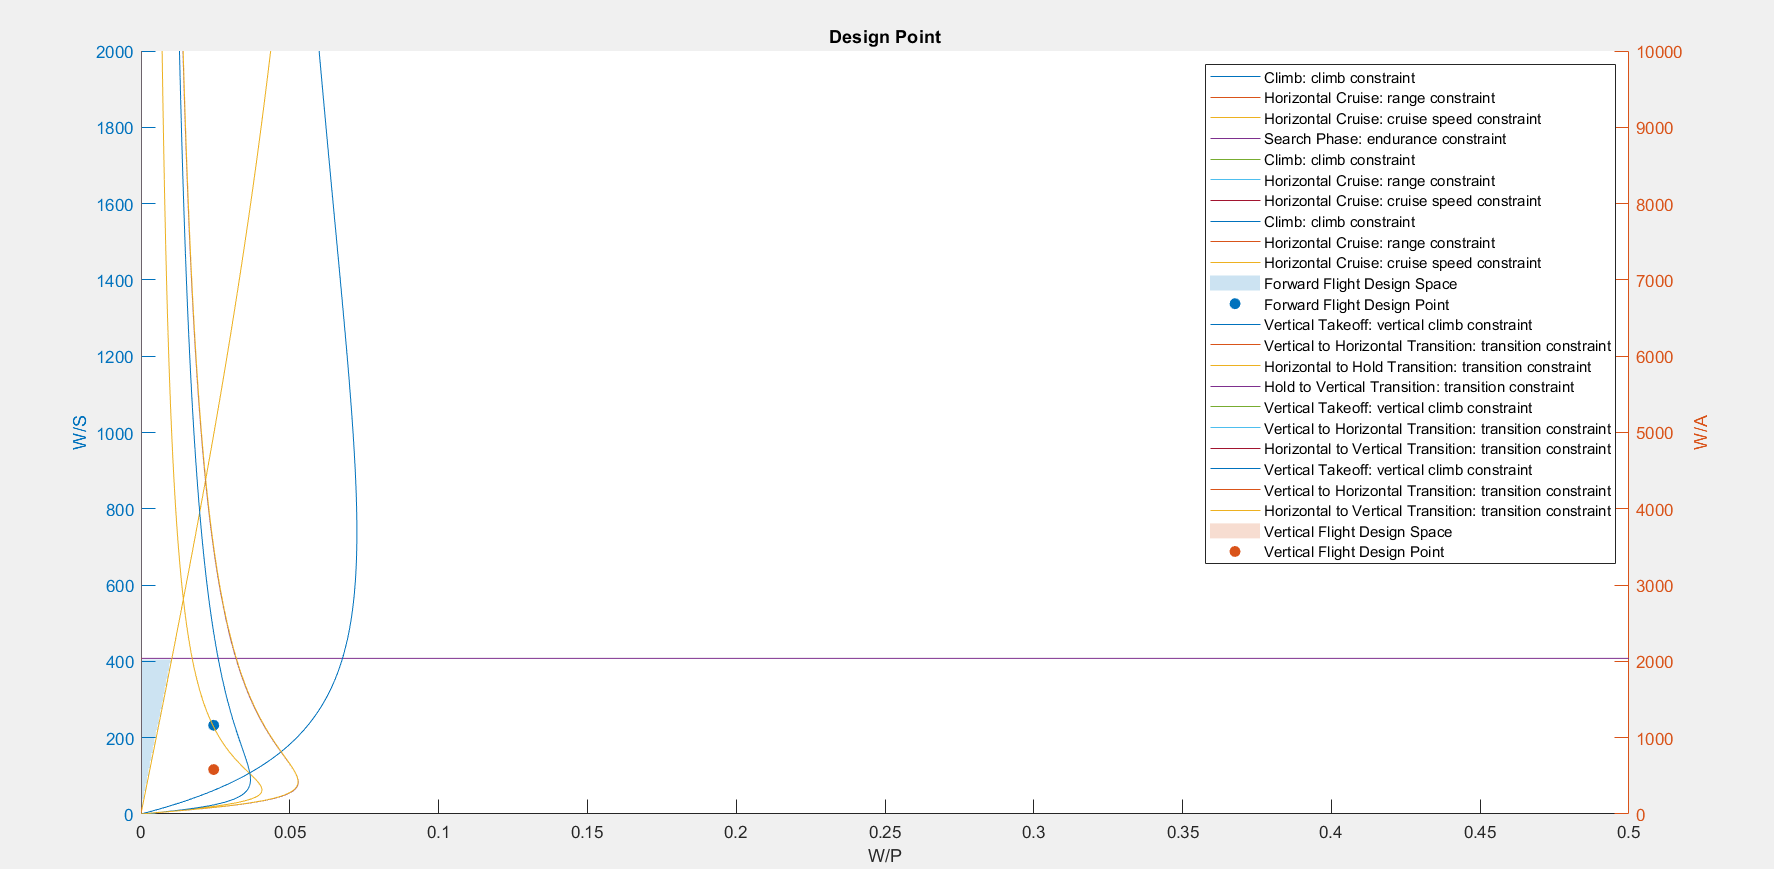
\includegraphics[width=\textwidth]{Imagens/secondplot_designpoint.PNG}
        \caption{Design Point}
        \label{}
    \end{subfigure}
    \hfill
    \begin{subfigure}[h]{0.70\textwidth}
        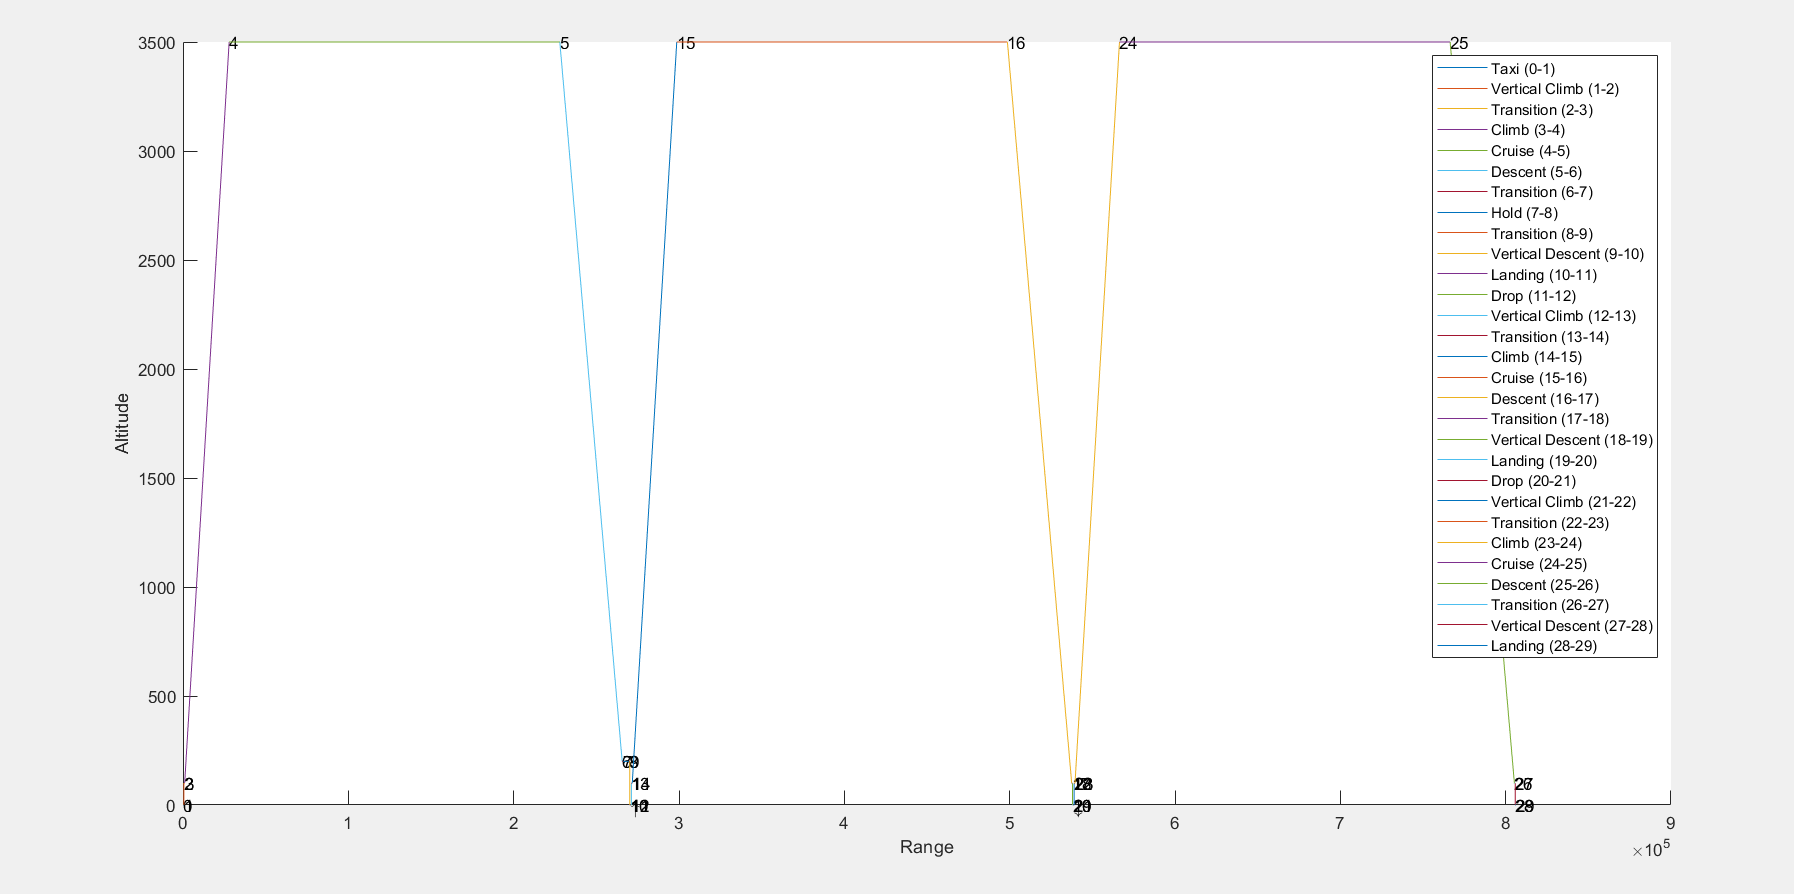
\includegraphics[width=\textwidth]{Imagens/secondplot_misson.PNG}
        \caption{Missão}
        \label{}
    \end{subfigure}
    \caption{Segundo Plot gerado pelo programa}
    \label{firstplot}
\end{figure}
\FloatBarrier
Este foi considerado uma melhor que o anterior, dado a presença de mais linhas, indicado a correção dum erro, bem como a valores de W/P mais perto da origem, ou seja, menores, para ambos os pontos. Isto significa que foi conseguido um compromisso onde é conseguido maior potência com menor peso.\par
É de notar que, no ficheiro json, as energy networks foram alteradas de forma a estarem devidamente formatadas. A "Hybrid Energy Network" foi a que sofreu maiores alterações. Primeiramente, foi adicionado ao turboshaft "brake\_specific\_fuel\_consumption", dado que o matlab o pedia; foi utilizado o valor default do programa. É importante, desde já, informar que este valor está errado, segundo valores históricos. Esta informação é explicitada e justificada devidamente na secção referente à semana 7, dado que só aí foi descoberto que o valor default estava em unidades imperiais e não SI. Segundamente, foi utilizado propellers como fim desta network, sendo-lhes adicionado: rotor\_solidity, base\_drag\_coefficient e induced\_power\_factor. É de notar que nos ficheiros json, estes valores estão apenas presentes nos rotores, e não nas propelles e que o programa esperara o uso de rotores em certos troços onde esta network foi utilizada, o que explica a necessidade de adicionar estes parâmetros. As propellers foram substituídas por rotores numa próxima semana. Notar que tal deveu-se tanto ao desconhecimento da nossa parte por a terminologia utilizada, dada nunca ter sido antes utilizada, bem como da falta de documentação do programa.\par
É apresentado de seguida a tabela com os dados colocados no json, estando todos estes em SI.\par
\FloatBarrier 
 \begin{table}[h] 
 \begin{adjustbox}{width=1\textwidth} 
 \begin{tabular}{|c|c|c|c|}
 \hline 

\makecell{name: Crew ; \\ type: mass.point ; \\ mass: 200 ; \\ } & \makecell{name: Passengers ; \\ type: mass.point ; \\ mass: 500 ; \\ } & \makecell{name: Avionics ; \\ type: mass.point ; \\ mass: 5 ; \\ } & \makecell{name: Payload Bay ; \\ type: mass.point ; \\ mass: 10 ; \\ }\\ \hline \\ 
\makecell{name: Fuselage ; \\ type: fuselage ; \\ interf\_factor: 1.0 ; \\ diameter: 1.0 ; \\ length: 4.0 ; \\ mass: 800 ; \\ } & \makecell{name: Main Wing ; \\ type: wing.main ; \\ interf\_factor: 1.0 ; \\ aspect\_ratio: 7.0 ; \\ mean\_chord: 3.0 ; \\ oswald\_efficiency: 0.85 ; \\ airfoil:   type :  naca0012  \\   tc\_max : 0.15 \\   xc\_max : 0.3 \\   lift\_slope\_coefficient : 6.2 \\   cl\_max : 2.0  ; \\ sweep\_le: 10.0 ; \\ sweep\_c4: 15.0 ; \\ sweep\_tc\_max: 20.0 ; \\ mass: 200 ; \\ } & \makecell{name: Horizontal Tail ; \\ type: wing.htail ; \\ interf\_factor: 1.0 ; \\ aspect\_ratio: 5.0 ; \\ mean\_chord: 0.5 ; \\ oswald\_efficiency: 0.85 ; \\ airfoil:   type :  naca0012  \\   tc\_max : 0.15 \\   xc\_max : 0.3 \\   lift\_slope\_coefficient : 6.2 \\   cl\_max : 2.0  ; \\ sweep\_le: 10.0 ; \\ sweep\_c4: 15.0 ; \\ sweep\_tc\_max: 20.0 ; \\ mass: 50 ; \\ } & \makecell{name: Vertical Tail ; \\ type: wing.vtail ; \\ interf\_factor: 1.0 ; \\ aspect\_ratio: 5.0 ; \\ mean\_chord: 1.0 ; \\ oswald\_efficiency: 0.85 ; \\ airfoil:   type :  naca0012  \\   tc\_max : 0.15 \\   xc\_max : 0.3 \\   lift\_slope\_coefficient : 6.2 \\   cl\_max : 2.0  ; \\ sweep\_le: 10.0 ; \\ sweep\_c4: 15.0 ; \\ sweep\_tc\_max: 20.0 ; \\ mass: 50 ; \\ }\\ \hline \\ 
\makecell{name: Turboshaft ; \\ type: engine.prop ; \\ efficiency: 0.8 ; \\ mass: 100 ; \\ max\_power: 210000 ; \\ } & \makecell{name: 4-stroke Piston Engine ; \\ type: engine.prop ; \\ efficiency: 0.8 ; \\ mass: 100 ; \\ max\_power: 200000 ; \\ } & \makecell{name: Jet Engine ; \\ type: engine.jet ; \\ mass: 200 ; \\ max\_power: 120000 ; \\ } & \makecell{name: Battery ; \\ type: energy.electric ; \\ specific\_energy: 360000.0 ; \\ efficiency: 0.9 ; \\ reserve: 0.2 ; \\ mass: 0 ; \\ }\\ \hline \\ 
\makecell{name: Fuel Tank ; \\ type: energy.fuel ; \\ reserve: 0.06 ; \\ mass: 0 ; \\ } & \makecell{name: Rotor ; \\ type: driver.rotor.main ; \\ number: 2 ; \\ number\_blades: 5 ; \\ radius: 2 ; \\ rotor\_solidity: 0.08 ; \\ induced\_power\_factor: 1.15 ; \\ base\_drag\_coefficient: 0.02 ; \\ tip\_velocity: 240.1 ; \\ efficiency: 0.6 ; \\ mass: 20 ; \\ } & \makecell{name: Propeller ; \\ type: driver.rotor ; \\ number: 2 ; \\ number\_blades: 4 ; \\ radius: 2.3 ; \\ tip\_velocity: 240.1 ; \\ efficiency: 0.6 ; \\ mass: 10 ; \\ } & \makecell{name: Gearbox ; \\ type: gearbox ; \\ efficiency: 0.95 ; \\ mass: 5 ; \\ }\\ \hline \\ 
\makecell{name: Generator ; \\ type: generator ; \\ efficiency: 0.96 ; \\ mass: 50 ; \\ } & \makecell{name: Electric Motor ; \\ type: engine.prop ; \\ number: 3 ; \\ efficiency: 0.97 ; \\ mass: 50 ; \\ max\_power: 200000 ; \\ } &  & \\ \hline \\ 
\end{tabular} 
 \end{adjustbox} 
 \end{table} 
 \FloatBarrier 


\par
O design apresentado acima, apesar de se apresentar como uma primeira base sólida, teve três problemas, ambos na missão: valores errados/irrealistas na missão; fases de missão erradas; e o uso de energy networks não suportadas.\par
O primeiro é caracterizado pelo o uso de velocidades demasiado elevadas, bem como de transition angles errados (devido a desconhecimento de como o programa interpretava esta valor). Além de tal, a search fase foi entendida como incorretamente caracterizada. Esta era descrita no json como uma hold, ou seja, voar a velocidade abaixo da de cruise, e foi visionada como a aeronave a voar a baixa velocidade com os motores tilted no ângulo mais efficiente, sendo, assim, mais efficiente que um simples hover dado a sustentação adicional dada pelas asas. No entanto, o programa entende que apenas a sustentação das asas é importante para neste mode de operação, pelo que é necessária uma velocidade alta para não entrar em stall. Isto é traduzido no programa como a existência duma linha vertical no plot do design point (W/S,W/A) baixa, reduzindo largamente a área. De forma a corrigir isto e gerar valores mais realista, foi mudado para hover. Entendemos este modo como uma estimativa conservativa, dada que a search phase pode ser realizada como anteriormente visionada na mesma, sendo, na realidade, mais eficiente que um simpls hover; ou seja, a limitação imposta pelo hover continua a ser maior que a real. Estas mudanças podem ser sumarizadas por:\par
\begin{itemize}
    \item Vertical take off velocity: 4 m/s
    \item Transition: 45º
    \item Hold changed to hover for search phase
    \item Search phase: 35 m/s
    \item Cruise velocity: 98 m/s
\end{itemize}
Por útlimo, vertical take off and landing não é suportado com combustível. Era assumido, no desenvolvimento projeto até aqui, dada a existência de múltiplos veículos capazes de realizar uma descolagem/aterragem com combustível, que este seria suportado no programa. É devido a tal que nunca se falou de descolagens verticais com baterias. No entanto, dada a falta de estimativas empíricas para fix wing aircraft presentes na literatura, não só não está presente no programa, como não foi possível implementá-la. Tal foi discutido com um dos criadores do programa, numa chamada por zoom de uma hora, numa tentativa de entender o que o programa suporta e quais a soluções possíveis. Foi-nos recomendados ceder ao uso de baterias ou encontrar relações empíricas, sendo-nos oferecida ajuda para serem implementadas. Dado que a nossa procura, ao longo da semana, foi infrutífera, escolhemos, reiterando, usar baterias.\par
Com estas mudanças, foi conseguido o seguinte design point:
\FloatBarrier
\begin{figure}[h]
    \centering
    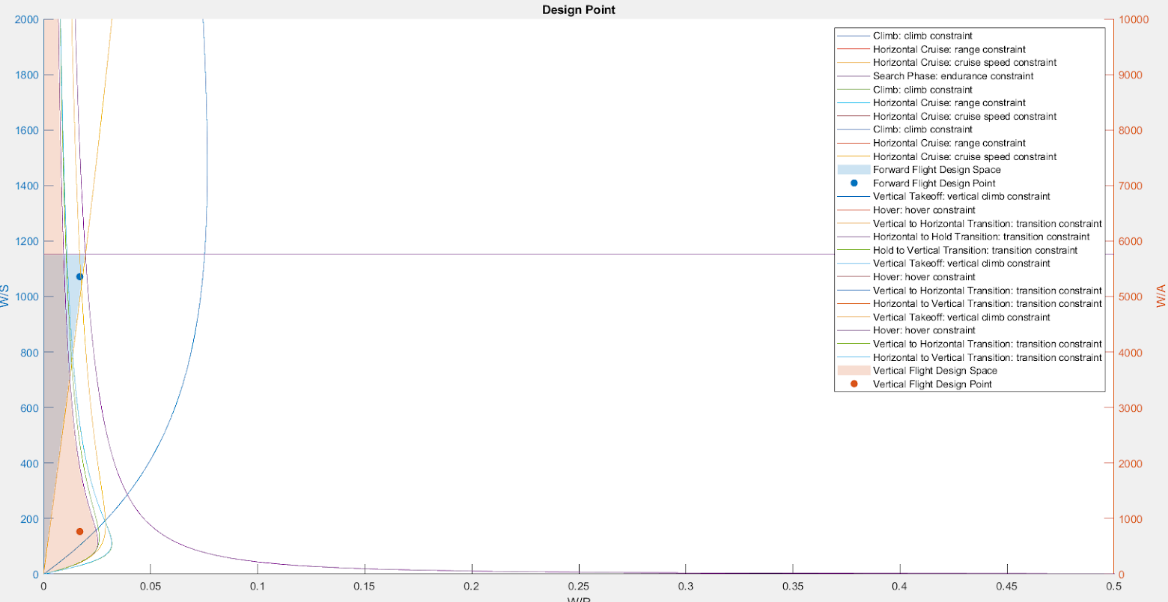
\includegraphics[width=\textwidth]{Imagens/semana4 powerpoint designpoint.png}
    \caption{Desgin Point final semanal- Semana 4}
    \label{designescolhido}
\end{figure}
\FloatBarrier
{\large\textbf{Colocar designs intermedios e tal; esta semana foi um inferno e precisamos de transmitir isso bem}}